\subsection{Page conditioning and line segmentation}
\label{sec:des-seg}
The recogniser needs one line of text at a time. A photographed page can contain shadows, rotation and strokes extending between lines. This stage prepares the page and returns ordered line crops while preserving the shape and spacing of the writing.

\subsubsection{Lighting normalisation and ink extraction}
A single brightness threshold can mistake a shadow for ink or lose pale strokes. The design compares each pixel with its local background, following the local comparison used in adaptive thresholding~\cite[pp.~2--3]{bradley2007}. Analysis uses a half-resolution grey image formed by averaging $2\times2$ blocks. The full-resolution page is retained for the final crops.

\paragraph{Estimating the local background.}
The background $B_r$ is the mean of a square window of radius $r$ around each grey pixel. The implemented radius is $r=\max(8,\min(40,\operatorname{round}(H/41)))$, where $H$ is working-image height. A summed-area table $S$ gives each window sum from four accesses~\cite[p.~2]{bradley2007}.
\begin{equation}
\Sigma_{[y_0,y_1)\times[x_0,x_1)}=
S(y_1,x_1)-S(y_0,x_1)-S(y_1,x_0)+S(y_0,x_0).
\label{eq:des-integral}
\end{equation}

The window area divides this sum to give $B_r$. Edge replication avoids darkening the image boundary with artificial zero padding. This calculation is independent of window size once the prefix table is available.

\paragraph{Separating ink from paper.}
Dividing grey intensity $G$ by its local background gives ratio $R$. Ink has a lower ratio than paper. The binary mask $M$ retains pixels below threshold $t^*$.
\begin{equation}
R(y,x)=\frac{G(y,x)}{\max[B_r(y,x),1]},\qquad
M(y,x)=\mathbf{1}[R(y,x)<t^*].
\label{eq:des-ratio}
\end{equation}

The denominator floor avoids division by zero. Otsu's criterion selects the threshold by maximising the separation between two histogram classes~\cite{otsu1979}. The class masses are $\omega_0,\omega_1$, with mean bin indices $\mu_0,\mu_1$.
\begin{equation}
t^*=\arg\max_t\ \omega_0(t)\omega_1(t)
\bigl[\mu_0(t)-\mu_1(t)\bigr]^2.
\label{eq:des-otsu}
\end{equation}

The software uses 256 bins over the clipped ratio range 0 to 1.2. Applying the threshold to a brightness ratio makes the decision less sensitive to gradual shadows than applying it directly to the grey image.

\paragraph{Calculation on an actual page.}
The recorded Owen01 example has pixel intensity 100 and local background 161.43, giving $R=0.62$. Its selected threshold is 0.80, so the pixel is retained as ink. Owen01 provides one traceable example throughout this explanation, rather than an average or a selected worst case. The prefix values and threshold calculation are retained in Appendix~\ref{app:worked-design-calculations}.

\subsubsection{Page orientation and skew correction}
A quarter turn changes the line axis, while a small rotation changes the slope of lines on that axis. The software first compares the fraction of nearly empty rows before and after a $90^\circ$ rotation. A turn requires a score improvement by a factor of 1.35, avoiding unnecessary rotation when the evidence is weak.

Fine deskewing then tests seventeen angles from $-4^\circ$ to $+4^\circ$ in $0.5^\circ$ steps. For each angle, $p_\theta(y)$ is the projected row ink count. Concentrating ink into distinct rows increases the squared-profile objective~\cite{postl1986}.
\begin{equation}
\theta^*=\arg\max_\theta\sum_y p_\theta(y)^2,\qquad
p_\theta(y)=\sum_x M_\theta(y,x).
\label{eq:des-skew}
\end{equation}

The search maps ink coordinates onto candidate rows in a further reduced mask. Only the selected rotation is applied to the full and working grey images, after which the mask is rebuilt. The Owen01 trace selects $+1.0^\circ$, with the trial scores retained in Appendix~\ref{app:worked-design-calculations}.

\subsubsection{Line detection and separation}
Line centres locate the writing, while curved boundaries separate overlapping ascenders and descenders. A straight horizontal cut can split these strokes even when they belong to different lines.

\paragraph{Removing marks and locating line centres.}
A preliminary line pitch $P$, meaning the estimated spacing between text lines, sets the scale for filtering page surrounds and printed rules. Horizontal and vertical run limits are 1.25 and 1.4 pitches. The pitch is estimated again after these marks and artifact components have been removed. A long handwritten underline can also meet a rule-removal condition.

The final smoothed row profile supplies candidate peaks above 6\% of its maximum. Median peak spacing gives the preferred pitch, with a lower bound based on component height. Autocorrelation and component height provide fallbacks. Centres are selected by peak strength with at least $0.6P$ separation. Optional shallow-valley merging is disabled by default.

\paragraph{Finding a boundary between lines.}
A boundary follows a low-cost path across each gap. The local cost combines a strong penalty for crossing ink with a weaker attraction towards midpoint $y_m$, scaled by half-gap height $h_g$.
\begin{equation}
C(y,x)=4\widetilde M(y,x)
+0.012\left(\frac{y-y_m}{h_g}\right)^2.
\label{eq:des-seamcost}
\end{equation}

Here $\widetilde M$ is the mask after morphological closing, a dilation followed by erosion~\cite[p.~541]{haralick1987}. Closing with radius $\max(2,\lfloor0.07P\rfloor)$ fills narrow breaks that could otherwise let the boundary enter a stroke. The weights are project choices. Dynamic programming then finds the path using accumulated cost $D$~\cite[p.~3]{avidan2007}.
\begin{equation}
D(y,x)=C(y,x)+\min_{|d|\leq s}
\{D(y+d,x-1)+0.02|d|\}.
\label{eq:des-seam}
\end{equation}

The allowed row change is $s=7$ per column. The $0.02|d|$ term discourages unnecessary vertical movement. Backtracking from the lowest final cost returns the seam. The worked recurrence and six-gap coefficient check are in Appendix~\ref{app:worked-design-calculations} and Appendix~\ref{app:des-seam-sweep}.

Figure~\ref{fig:des-seam-example} shows one gap from Abhinav01. It was selected for the largest reduction in crossed ink on that page. The seam crosses one working-image ink pixel, compared with 64 for the straight midpoint cut. The lower panel shows the cost field that makes the seam bend around the writing. The second example and complete original figure are in Appendix~\ref{app:extended-design-figures}.
\begin{figure}[H]\centering
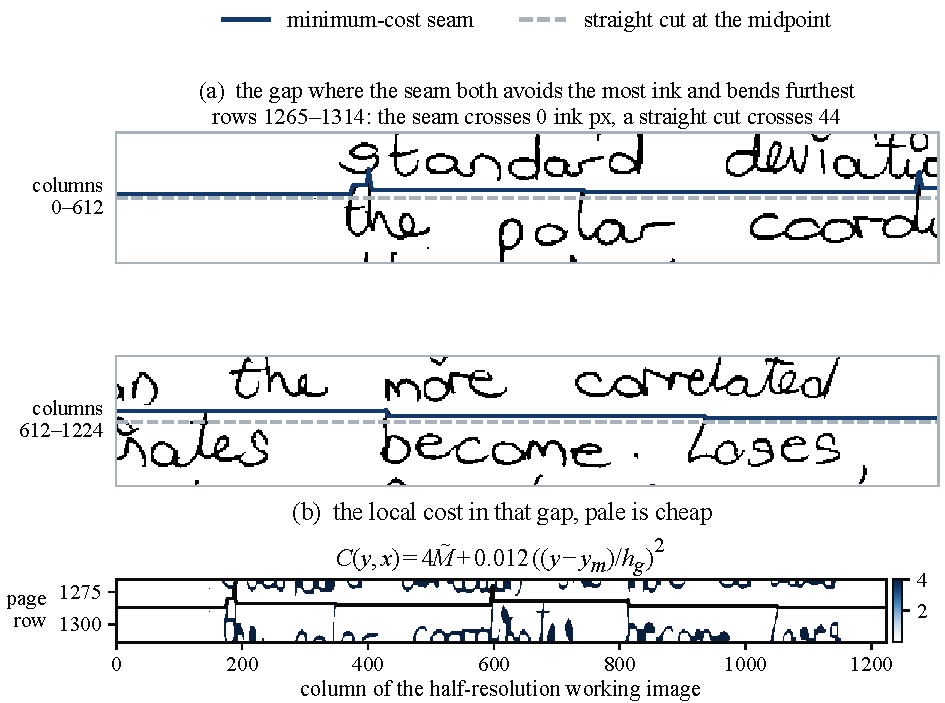
\includegraphics[width=\linewidth]{Figures/design-seam-two-panels.pdf}
\caption{Seam path and its cost field.}
\label{fig:des-seam-example}
\end{figure}

\subsubsection{Assigning ink to the correct line}
A seam divides the page into bands, but a dot or descender can still fall into its neighbour's band. Eight-connected components, found using row runs and union operations, provide a second check~\cite[pp.~476--479]{rosenfeld1966}.

For each component, a band containing at least 15\% of its in-band ink is substantial. The uppermost substantial band supplies the reference owner for eligible small-piece corrections. If none qualifies, the largest overlap is used. Large components retain their seam assignments except for the narrow-tail and small-piece rules.

For example, an \texttt{i} dot may lie above the seam while its stem supports assignment to the lower line. Raw components are revisited because closing may join the dot to an unrelated stroke. Enclosed-ring and residual-fragment checks handle further detached pieces. Algorithm~\ref{alg:des-ownership} gives this order, with $O$ storing each pixel's line index.
\begin{designalgorithm}
\caption{Refining seam bands into ink ownership}
\label{alg:des-ownership}
\prequire{Ink mask $M$, components $\mathcal C$, seams, centres and pitch $P$.}
\begin{designpseudo}
\pstate{0}{\textbf{for each} component $C\in\mathcal C$ \textbf{do}}
\pstate{1}{Count overlap $a_{C,n}$ with each seam band $n$}
\pstate{1}{$S\leftarrow\{n:a_{C,n}\geq0.15\sum_j a_{C,j}\}$}
\pstate{1}{Choose topmost $S$ as reference owner, or maximum overlap if $S=\varnothing$}
\pstate{1}{Correct eligible narrow tails and small pieces; reject remote specks}
\pstate{1}{Associate compact dots with plausible stems using pitch-scaled guards}
\pstate{0}{\textbf{end for}}
\pstate{0}{$O\leftarrow$ corrected ownership, preserving large-piece seam assignments}
\pstate{0}{\textbf{for each} raw component near a neighbouring line \textbf{do}}
\pstate{1}{\textbf{if} detached-dot or enclosed-ring guards pass \textbf{then}}
\pstate{2}{Transfer eligible pixels to the supported stem's line; protect correction}
\pstate{1}{\textbf{end if}}
\pstate{0}{\textbf{end for}}
\pstate{0}{Reassign residual fragments lacking their own body-band support}
\pstate{0}{\textbf{return} $O$; excluded pixels retain no line index}
\end{designpseudo}
\end{designalgorithm}

Figure~\ref{fig:vt-ownership} shows the three largest corrections on Abhinav01. The boxes mark the affected pieces and colour shows the assigned line. The complete page has 462 reassigned pixels. This count shows where the rules act, without treating reassignment alone as proof of correct ownership.
\begin{figure}[H]\centering
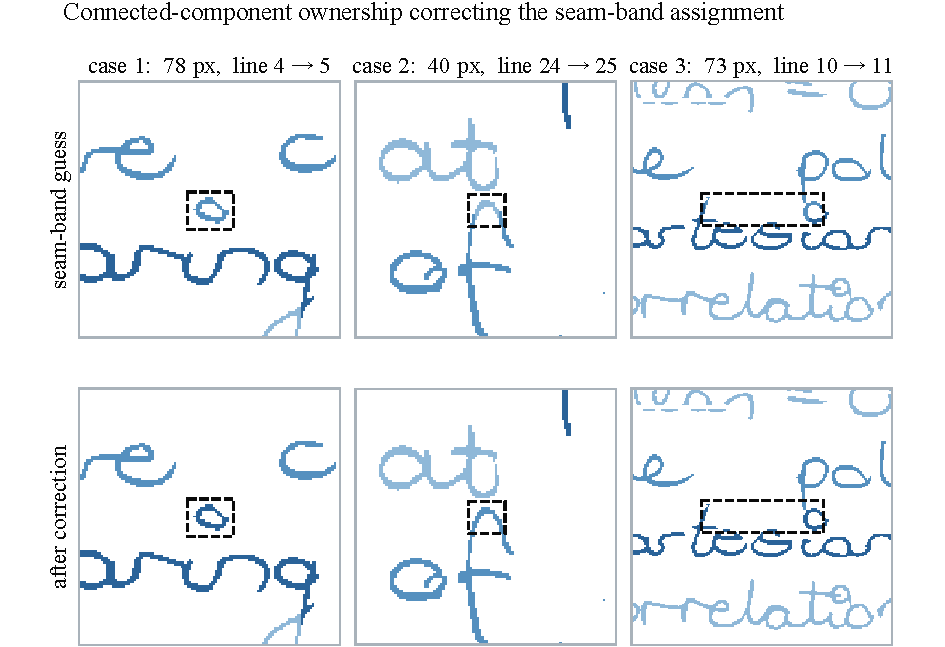
\includegraphics[width=\linewidth]{Figures/VisualTests/T27_ownership_corrections.pdf}
\caption{Ink ownership before and after correction.}
\label{fig:vt-ownership}
\end{figure}

\subsubsection{Preparing the classifier crops}
Crops are built from the full-resolution image after ownership is settled. A soft ink mask avoids jagged edges, while a separate nearest-neighbour ownership exclusion keeps neighbouring ink out. Contrast stretching and a darkness exponent of 0.55 strengthen faint retained strokes.

The solid-crop guard rejects a line only when its dark-pixel fraction exceeds both 15\% and three times the page median. If every crop would be rejected, the input list is retained. The guard therefore reduces solid-shadow crops without establishing that every remaining crop is valid.

The classifier canvas is $64\times640$ pixels. A common scale preserves the proportions of a crop of height $h$ and width $w$.
\begin{equation}
a=\min\left(\frac{64}{h},\frac{640}{w}\right),\qquad
(h',w')\simeq(ah,aw).
\label{eq:des-fit}
\end{equation}

For the archived $156\times2170$ Owen line, $a\simeq0.295$ gives a $46\times640$ image. It is left-aligned, vertically centred and padded white. A very long line loses vertical detail when the width limit controls this scale.

\subsubsection{Complete processing sequence and output}
Figure~\ref{fig:des-seg-stages} follows the page from lighting correction to ink extraction, line boundaries and final crops. These views show where a stroke was removed or assigned to another line. Algorithm~\ref{alg:des-segment} gives the full sequence after the individual operations described above.
\begin{figure}[H]\centering
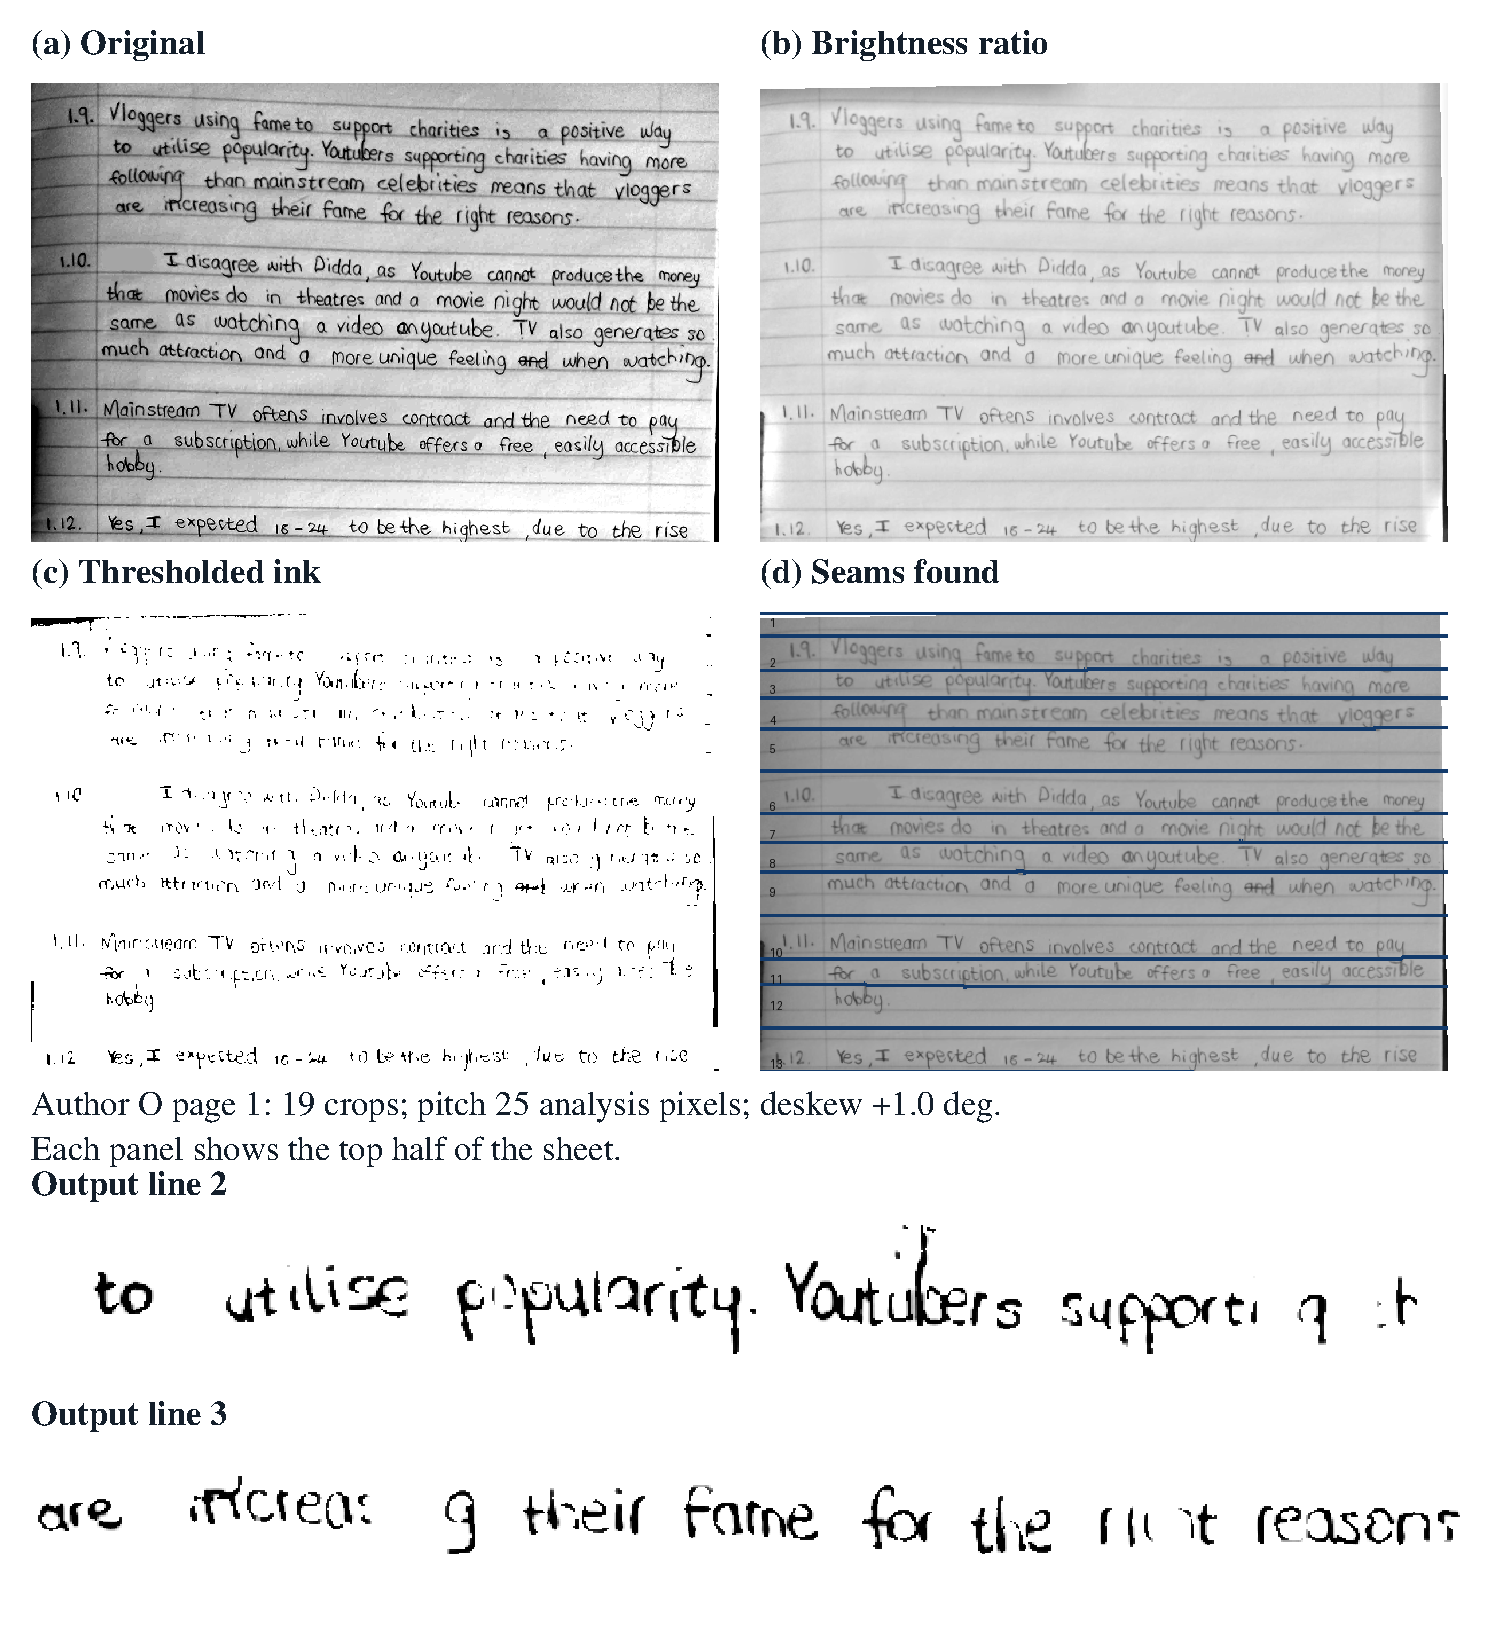
\includegraphics[width=\linewidth]{Figures/design-segmentation-stages.pdf}
\caption{Page preparation and line extraction.}
\label{fig:des-seg-stages}
\end{figure}

In the algorithm, $G_f,G_h$ are the full and half-resolution grey images, $R$ is the brightness ratio and $M$ is the ink mask. Pitch $P$, centres $c$ and seams $b$ define the lines. The output $\mathcal L$ contains the ordered crops, classifier views and bounding boxes.
\begin{designalgorithm}
\caption{Photographed page to ordered line crops}
\label{alg:des-segment}
\prequire{Grey page on its chosen line axis.}
\pensure{Ordered full-resolution crops, coordinates and diagnostics.}
\begin{designpseudo}
\pstate{0}{$(G_f,G_h,M,R,\theta)\leftarrow\operatorname{Deskew}(G)$}
\pstate{0}{$M\leftarrow\operatorname{RemovePrintedStructure}(M,G_h)$}
\pstate{0}{$(M,\mathcal C)\leftarrow\operatorname{DropArtifactPieces}(M,R)$}
\pstate{0}{$(P,c)\leftarrow\operatorname{LineCentres}(M)$}
\pstate{0}{$b\leftarrow\operatorname{SeamCuts}(M,c,P)$}
\pstate{0}{$O\leftarrow\operatorname{AssignOwnership}(M,\mathcal C,b,c,P)$}
\pstate{0}{$\mathcal L\leftarrow\varnothing$; normalise full-resolution brightness}
\pstate{0}{\textbf{for each} line index $n$ \textbf{do}}
\pstate{1}{$C_n\leftarrow\operatorname{BuildLineCrop}(n,O,G_f,P)$}
\pstate{1}{\textbf{if} $C_n$ has sufficient ink and height \textbf{then}}
\pstate{2}{Append $C_n$, its fixed-canvas view and bounding box to $\mathcal L$}
\pstate{1}{\textbf{end if}}
\pstate{0}{\textbf{end for}}
\pstate{0}{$\mathcal L\leftarrow\operatorname{DropSolidCrops}(\mathcal L)$; renumber retained crops}
\pstate{0}{\textbf{return} $\mathcal L$, seams, ratio image and diagnostics}
\end{designpseudo}
\end{designalgorithm}

After cropping, the reader compares up to three sampled lines in both directions to distinguish upright from upside-down writing. It chooses the higher mean frame log score, reuses those readings and reverses line order when needed. This heuristic can still fail when the reader is confidently wrong.

\subsubsection{Segmentation verification and limitations}
\label{sec:des-segverify}
The native Owen01 page produces 20 crops for 20 labelled lines. Figure~\ref{fig:des-seg-variation} tests a harder sparse page photographed three times. The striped-shadow image gives three crops, the diffuse-shadow image four, and the changed-angle image 28. In the last case, gap scores of 0.379 and 0.400 give only a 1.054 ratio, below the 1.35 turn threshold. Fine deskewing cannot repair the missed quarter turn.
\begin{figure}[H]\centering
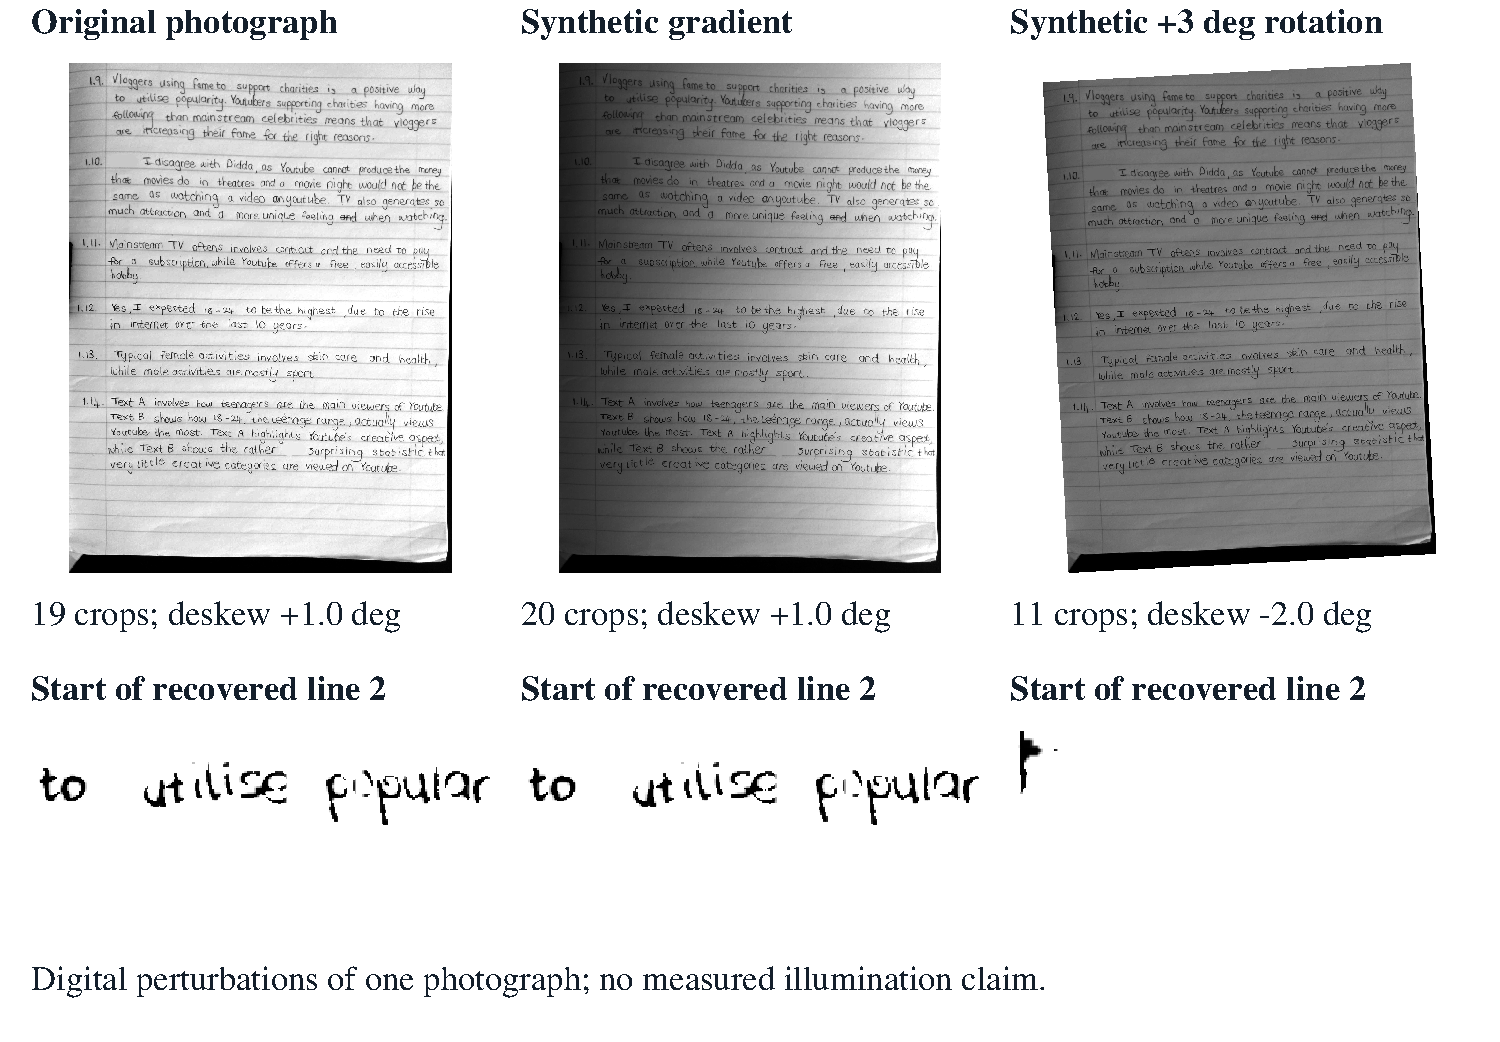
\includegraphics[width=\linewidth]{Figures/design-segmentation-variation.pdf}
\caption{Three captures of the same sparse page.}
\label{fig:des-seg-variation}
\end{figure}

These captures show failure conditions rather than a measured lighting range. Irregular spacing weakens pitch estimation, touching strokes can defeat ownership, and sparse pages provide little orientation evidence. A fixed mount and restrained page reduce perspective and curvature that a global rotation cannot correct. Appendix~\ref{app:des-visual-tests} retains the capture records and extended checks.
\FloatBarrier
